\documentclass{article}
\usepackage{lipsum}
% geometry package, control the margin of the article
\usepackage[margin = 1 in, left = 1.5 in, includefoot]{geometry}
% Header and Footer Stuff
\usepackage{fancyhdr} % fancyhdr package
\pagestyle{fancy}
% Clear previous head and foot style
\fancyhead{}
\fancyfoot{}
% Position the page number RHS of the footer
\fancyfoot[R]{ \thepage\ }
% Clear the header line
\renewcommand{\headrulewidth}{0pt}
% Keep the footer line
\renewcommand{\footrulewidth}{1pt}

% Graphics preamble
\usepackage{graphicx}% Import images
\usepackage{subcaption}
\usepackage{float} % Control float options
% Graphics preamble
\usepackage[numbers]{natbib}

% Maths preamble
\usepackage{amsmath}
% Maths preamble
\begin{document}
\begin{titlepage}
	\begin{center}
		\line(1,0){300}\\
		[0.25in]
		\huge{\textbf{ CSSA \LaTeX\ Notes}}\\
		[2mm]
		\line(1,0){200}\\
		[1.5cm]
		\textsc{\LARGE University of Cambridge}\\
		\textsc{\LARGE Using \LaTeX\ to Write a Simple Report}\\
		[8cm]
	\end{center}
	\begin{flushright}
		\textsc{\large CSSA. \\ A \LateX{} User\\
		20th Apr 2019}
	\end{flushright}
\end{titlepage}
\cleardoublepage
% Table of contents stuff
\pagenumbering{roman}
\tableofcontents
% \cleardoublepage
% List of figures, list of tables
\listoffigures
\listoftables

\thispagestyle{empty}
\addcontentsline{toc}{section}{\numberline{}List of Figures}
\addcontentsline{toc}{section}{\numberline{}List of Tables}
\cleardoublepage

% Main body stuff
\pagenumbering{arabic}
\setcounter{page}{1}

\cleardoublepage
\section{Introduction} 
This is the first line of the report. This report will show you how to use \LaTeX\\\
% Text holder here, show one paragraph of \lipsum
\lipsum[1]
\section{Second section}
This is the second section of this report.
\subsection{Sub section 1} 
This is the first sub section in this report.
\subsection{Sub section 2} 
This is the second subsection in this report.
\subsubsection{Sub sub section}
This is a sub sub section. Replace text here when you write your report.
\cleardoublepage
\section{Lists}
% Normal bullet point: itemized
\begin{itemize}
	\item This is our first line
	\item This is our second line and I am making it longer so that you can see how text wraps around automatically in \LaTeX
	\begin{itemize}
		\item A bullet within a bullet!
		\begin{itemize}
			\item More deeper
		\end{itemize}
	\end{itemize}
	\item [Title] blah blah blah
	\item [This is a longer title] blah blah blah
	\begin{enumerate}
		% Numberd lists
		\item \lipsum[1]
		% Just try to make the PDF looks okay for this presentation
		\item \lipsum[2]
	\end{enumerate}
\end{itemize}

\cleardoublepage
\section{Figures and Tables}
\subsection{Figures}
\begin{figure}[H]
	\centering
	
\includegraphics[width = \textwidth]{Figures/space.png}
	\caption{My desktop background}
	\label{fig}
\end{figure}
\subsection{Tables}
\begin{table}[H]
	\centering
	\caption{This is a very simple table}
	\begin{tabular}{l | c r}
		Name & University & Department \\\hline
		CSSA & Cambridge & Engineering \\
	\end{tabular}
	\label{tab}
\end{table}
Figure \ref{fig}. Table \ref{tab}.

\cleardoublepage
\section{Math equation}
Fractions, inline equation: $d = v_it + \frac{1}{2} \cdot at^2$\\
Brackets:
$$\left(\frac{1}{2}\right) \cdot 2 = 1$$ 
$$\left|-7 \right| = 7$$
$$x^{2^3}$$
\begin{eqnarray*}
    \sqrt{4} &\neq& 5 \\ 
    \pi &\approx& 3 \\
    \pi &\times& \sqrt{4} < 15
\end{eqnarray*}
\begin{equation}
	U(\alpha, \beta) = \frac{e^{jkz}}{j\lambda z}e^{j\frac{k(\alpha^2+\beta^2)}{2z}}\iint\left\{U(x,y)e^{j\frac{k(x^2+y^2)}{2z}}\right\}e^{-j\frac{2\pi}{\lambda z}(\alpha x+\beta y)}dxdy
	\label{eq:Fresnel}
\end{equation}
% Equation \ref{eq:FresnelDiffractionIntegralFomula} can be simplified as follows:
% \begin{equation}
% 	U(u,v) = \iint U(x,y)e^{-j2\pi(ux+vy)}dxdy
% 	\label{FourierTransformOfLight}
% \end{equation}
% Figure \ref{cubicAperture} and \ref{circularAperture} visualized a plane wave traversing a cubic or a circular aperture respectively.
% \begin{figure}[H]
% 	\begin{subfigure}{0.5\linewidth}
% 		% \centering
% 		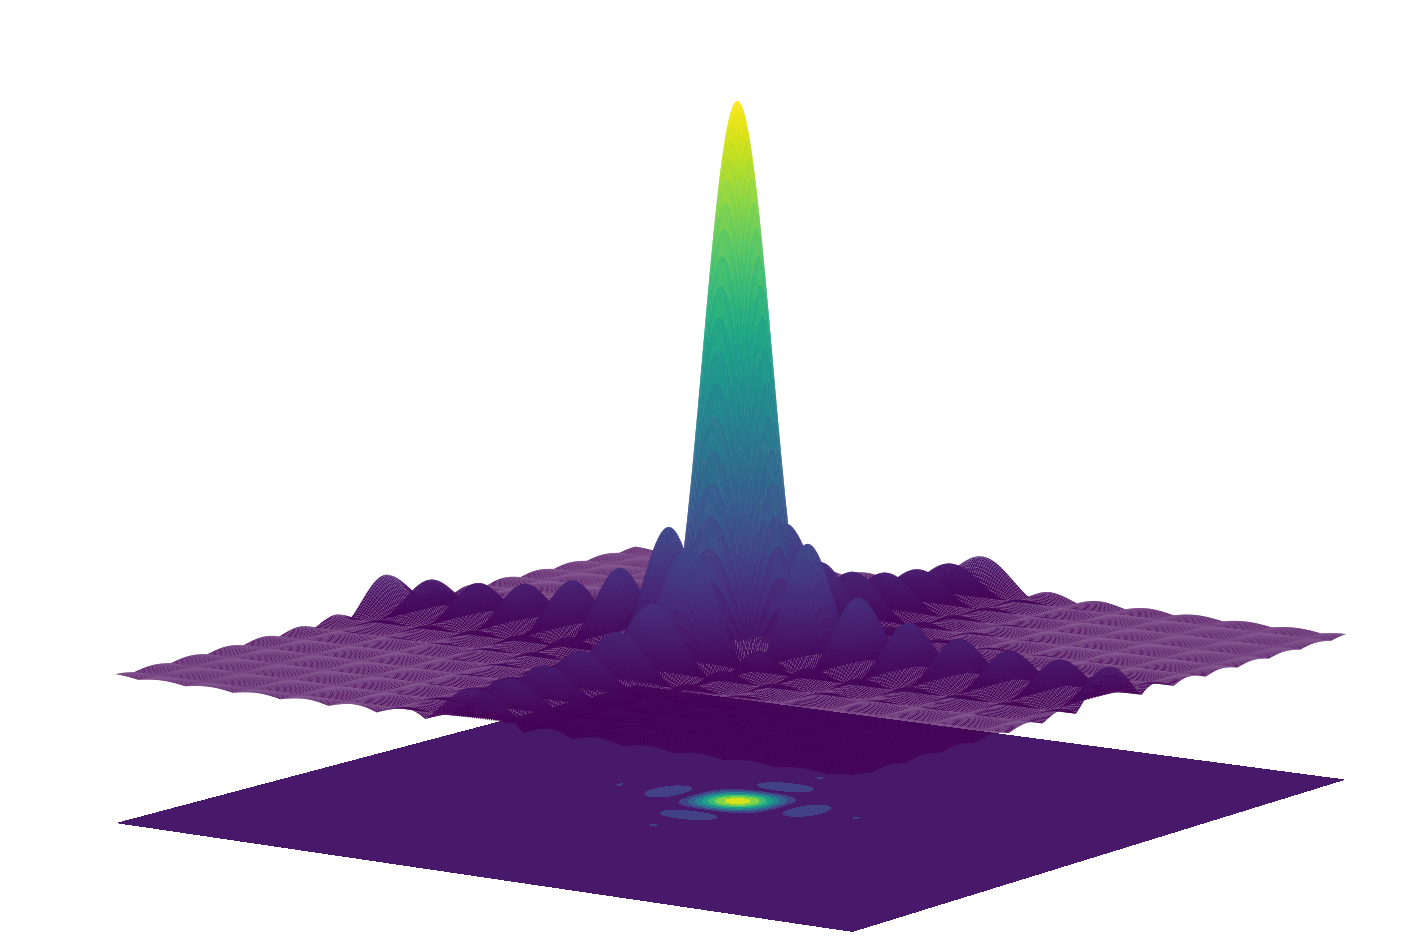
\includegraphics[width = \textwidth]{Figures/Cubic_aperture.png}
% 		\caption{cubic aperture}
% 		\label{cubicAperture}
% 	\end{subfigure}
% 	\begin{subfigure}{0.5\linewidth}
% 		% \centering
% 		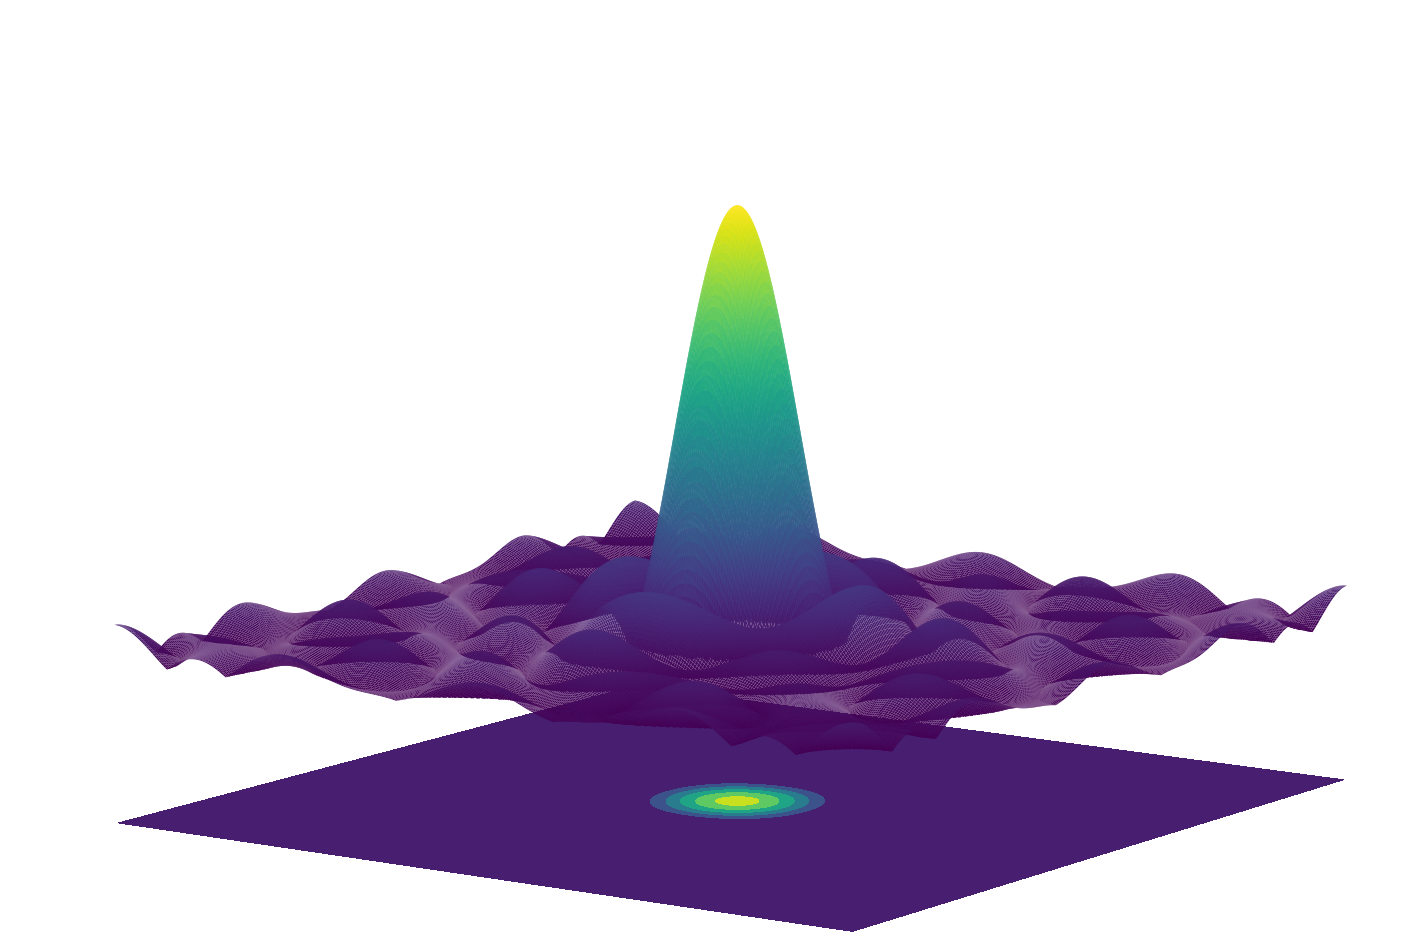
\includegraphics[width = \textwidth]{Figures/Circular_aperture.png}
% 		\caption{circular aperture}
% 		\label{circularAperture}
% 	\end{subfigure}
% \end{figure}
\cleardoublepage

\section{How to use refernces}
\lipsum[1]
\textbf{I'm citing a journal article} \cite{GaborHolography}.\\
\lipsum[2]
\textbf{I'm now citing a conference article} \cite{HardReview_84}.


\bibliographystyle{IEEEtran}
\cleardoublepage
\bibliography{References/references.bib}
\addcontentsline{toc}{section}{\numberline{}References}

\cleardoublepage
\appendix
\section{Some data}
This is the first appendix.  But I did not call
it Appendix~1, because I might want to add some
other appendix before it later.  In general it is
best to let \LaTeX{} do the numbering by itself,
and use cross-references.  That way, you won't
manually need to change any of your numbers if
you insert an extra section in the middle, or
delete one.

\lipsum[1]
\section{Some more data}
This is the second appendix.
\begin{figure}[H]
	\begin{subfigure}{0.5\linewidth}
		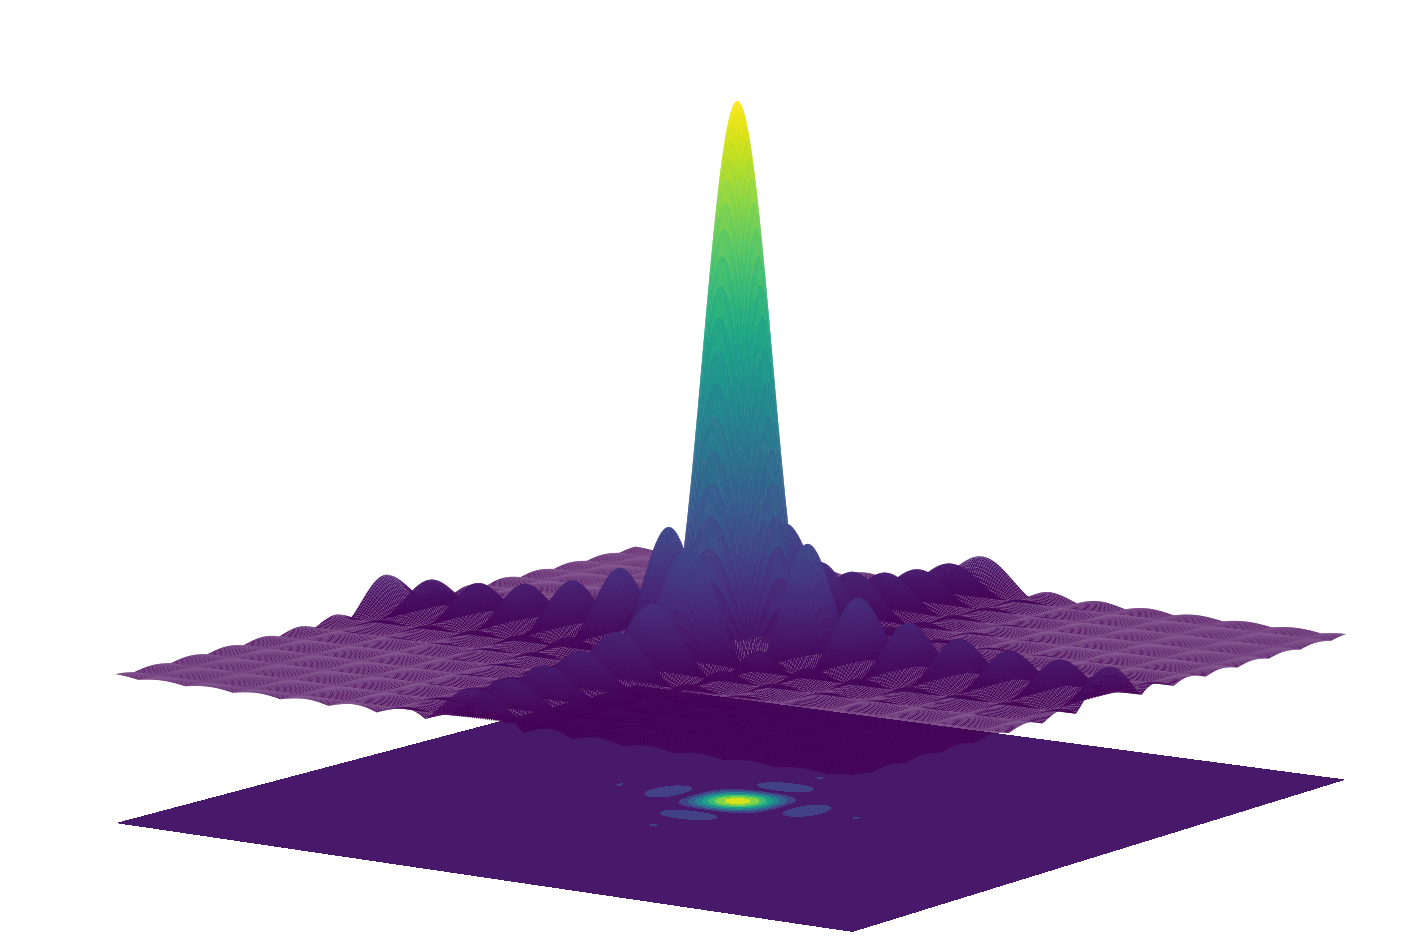
\includegraphics[width = \textwidth]{Figures/Cubic_aperture.png}
		\caption{cubic aperture}
		\label{cubicAperture}
	\end{subfigure}
	\begin{subfigure}{0.5\linewidth}
		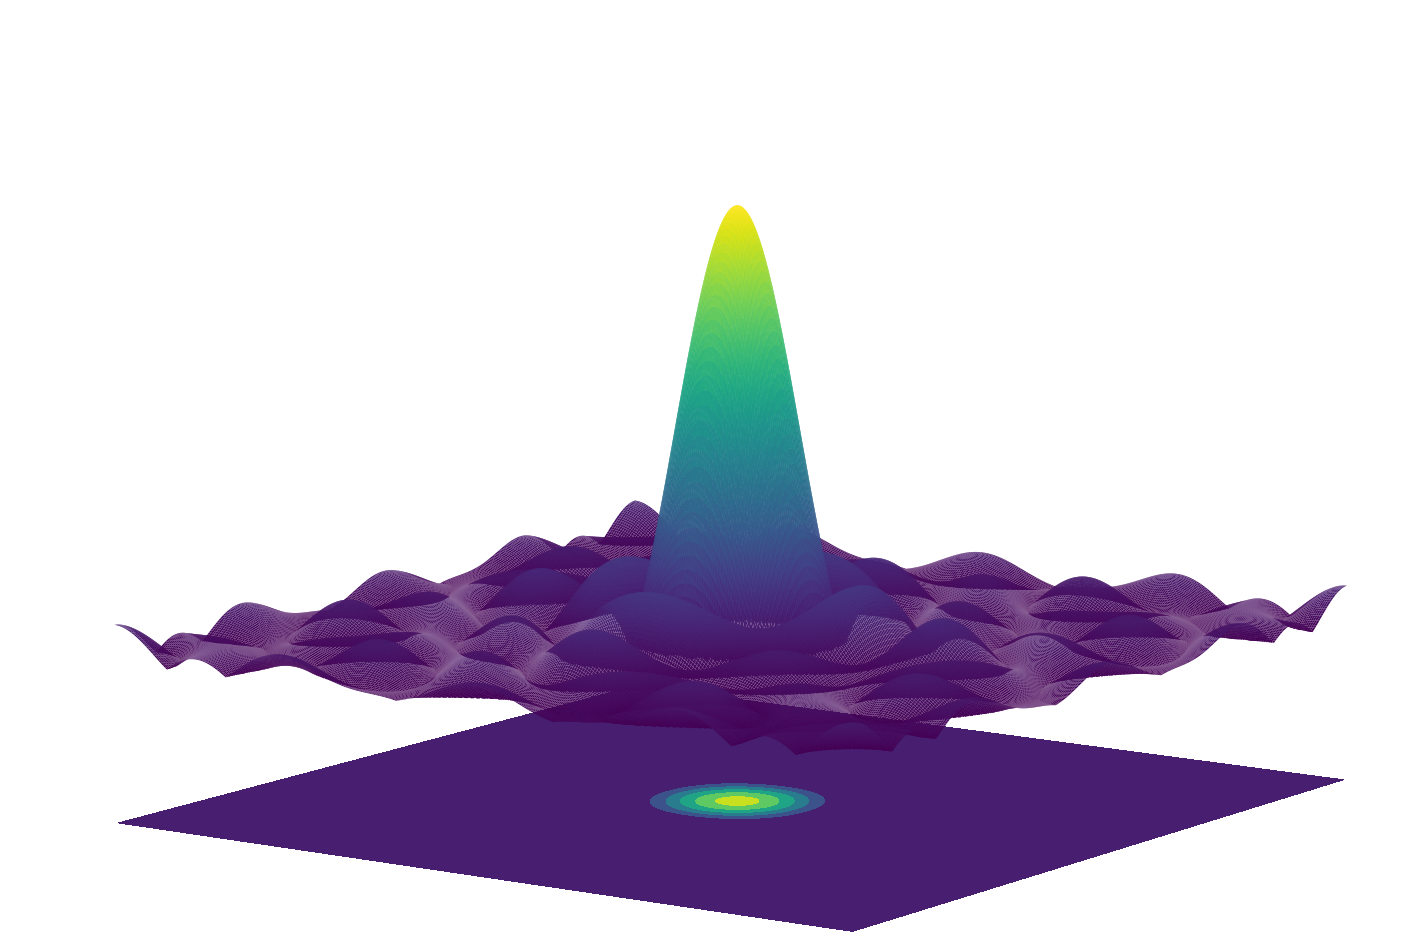
\includegraphics[width = \textwidth]{Figures/Circular_aperture.png}
		\caption{circular aperture}
		\label{circularAperture}
	\end{subfigure}
	\caption{Two figures}
\end{figure}

\end{document}
